\section{Kohonen Network}
1982 yılında Finli bilim adamı Teuvo Kohonen tarafından geliştirilmiştir. Yüksek boyutlu verileri görselleştirmek için kullanılır. 

\begin{figure}[h]
    \centering
    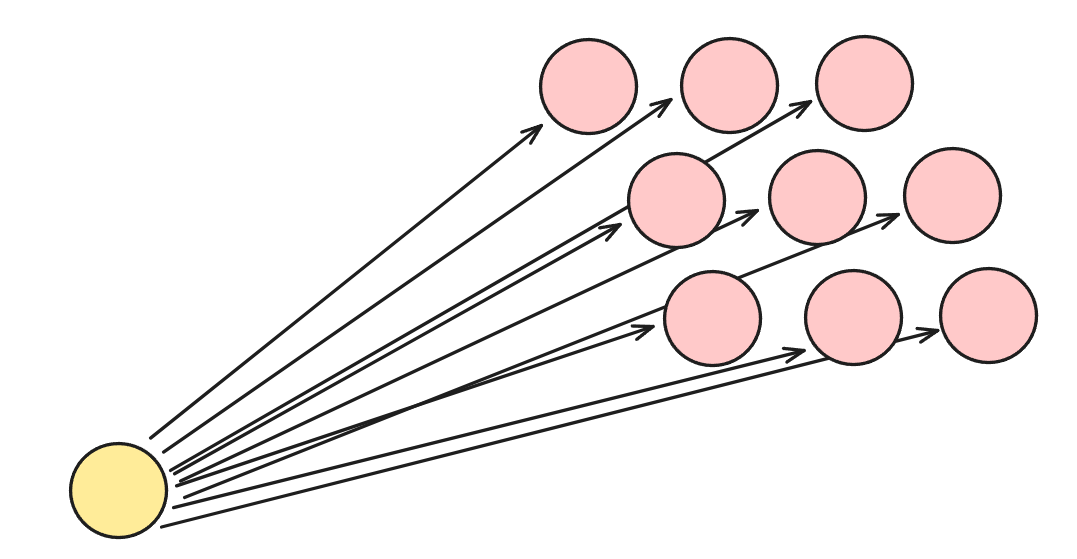
\includegraphics[width=1\textwidth]{images/kohonen_network.png}
    \caption{Kohonen ağı mimarisi.}
    \label{fig:enter-label}
\end{figure}

\subsection{Çalışma Adımları}
\begin{enumerate}
    \item Kohonen ağının her bir nöronu başlangıçta rastgele seçilen değerlere sahip bir vektörü temsil eder.
    \item Giriş verisiyle her bir nöronun benzerliği hesaplanır ve en yakın nöron bulunur. Bu nöron "kazanan" nöron olarak adlandırılır ve bu süreç "yarışma" süreci olarak bilinir.
    \item Kazanan nöronun ağırlıkları ve çevresindeki diğer nöronların ağırlıkları, giriş verisiyle uygun hale getirilerek kazanan nöron giriş verisine yaklaşır. Kazanan nöronun komşu nöronları da güncellenerek ağın daha homojen bir yapıya sahip olması sağlanır.
    \item Her iterasyonda öğrenme oranı azaltılarak ağırlıkların daha yavaş bir şekilde güncellenir. Bu aşırı uyumu önlemeye yardımcı olur.
\end{enumerate}

\newpage